%% LyX 2.1.4 created this file.  For more info, see http://www.lyx.org/.
%% Do not edit unless you really know what you are doing.
\documentclass[12pt,english]{article}
\usepackage[T1]{fontenc}
\usepackage[latin9]{inputenc}
\usepackage{amsmath}
\usepackage{amsthm}
\usepackage{graphicx}
\usepackage{esint}

\makeatletter
%%%%%%%%%%%%%%%%%%%%%%%%%%%%%% Textclass specific LaTeX commands.
\numberwithin{equation}{section}
\numberwithin{figure}{section}

%%%%%%%%%%%%%%%%%%%%%%%%%%%%%% User specified LaTeX commands.
\usepackage[margin=0.75in]{geometry} % see geometry.pdf on how to lay out the page. There's lots.
\usepackage{graphicx}
\usepackage{cleveref}
\usepackage{amsmath}
\usepackage{multirow}
\usepackage{listings}
\usepackage{color}
\usepackage{CJK}
\definecolor{mygreen}{RGB}{28,172,0}
\definecolor{mylilas}{RGB}{170,55,241}

\usepackage[latin9]{inputenc}
\usepackage{geometry}
\geometry{verbose}


\makeatletter
\@ifundefined{date}{}{\date{}}
\makeatother

%Fancy-header package to modify header/page numbering 
\usepackage{fancyhdr}
\pagestyle{fancy}
\lhead{\textbf{Ge/ESE 118}} %name of the course
\chead{\textbf{}} %topic of the homework set
\rhead{\textbf{Solution 4}} %number of the homework set
\lfoot{}
\cfoot{}
\rfoot{\thepage}


% Matlab script
\lstset{language=Matlab,%
      %basicstyle=\color{red},
  breaklines=true,%
  morekeywords={matlab2tikz},
  keywordstyle=\color{blue},%
  morekeywords=[2]{1}, keywordstyle=[2]{\color{black}},
  identifierstyle=\color{black},%}
  stringstyle=\color{mylilas},
  commentstyle=\color{mygreen},%
  showstringspaces=false,%without this there will be a symbol in the places where there is a space
  numbers=left,%
  numberstyle={\tiny \color{black}},% size of the numbers
  numbersep=9pt, % this defines how far the numbers are from the text
  emph=[1]{for,end,break},emphstyle=[1]\color{red}, %some words to emphasise
                                                      %emph=[2]{word1,word2}, emphstyle=[2]{style},    
}

\makeatother

\usepackage{babel}
\begin{document}

\subsection*{Problem 1 (graded by Yiran) 50 points}


\subsubsection*{(a) - 8 points}

The misfit function 
\begin{eqnarray*}
F(\boldsymbol{m}) & = & \sum_{i}\frac{(d_{i}-g_{i}(\boldsymbol{m}))^{2}}{2\sigma_{d}^{2}}
\end{eqnarray*}


Then, the posterior PDF

\begin{eqnarray*}
P(\boldsymbol{m}|\boldsymbol{d})\propto P(\boldsymbol{d}|\boldsymbol{m}) & \propto & \exp\left(-F(\boldsymbol{m})\right)\\
 & \approx & \exp\left(-F(\boldsymbol{m}_{0})-\bigtriangledown F(\boldsymbol{m}_{0})^{T}(\boldsymbol{m}-\boldsymbol{m}_{0})-\frac{1}{2}(\boldsymbol{m}-\boldsymbol{m}_{0})^{T}\boldsymbol{H(m}_{0})(\boldsymbol{m}-\boldsymbol{m}_{0})\right)
\end{eqnarray*}
 has the form of a multivariate Gaussian distribution, and the covariance
matrix is 
\begin{eqnarray*}
cov(\boldsymbol{m})=\boldsymbol{H}(\boldsymbol{m_{0}})^{-1}
\end{eqnarray*}
Note we want to know the covariance matrix when $m_{0}$ is the least
squares solution. 

In HW2, we didn't include the data error, and 
\begin{eqnarray*}
\hat{G}_{i,k}=\frac{\partial g_{i}}{\partial m_{k}}
\end{eqnarray*}


To include the data error

\begin{eqnarray*}
\boldsymbol{H}\approx\frac{\hat{\boldsymbol{G}}^{T}\hat{\boldsymbol{G}}}{\sigma_{d}^{2}}
\end{eqnarray*}


So we need to modify the hessian in HW2 by dividing $\sigma_{d}^{2}$
when calculate the model covariance matrix. 

(See MATLAB code) The output model covariance matrix is:
\begin{verbatim}
    0.0101   -0.0123    0.0095    0.0548    
   -0.0123    0.0198   -0.0156   -0.0853     
    0.0095   -0.0156    0.0237    0.1034     
    0.0548   -0.0853    0.1034    0.4985
\end{verbatim}
\selectlanguage{english}%

\subsubsection*{(b)- 8 points}

The covariance matrix calculated here will be similar to the Monte
Carlo simulation in HW2.

Diagonal element shows the variance of each parameter. The square
root of the diagonal elements gives the standard deviations: $\sigma_{x_{s}}=0.1006$,
$\sigma_{y_{s}}=0.1405$, $\sigma_{z_{s}}=0.1538$, $\sigma_{P}=0.7060$.
The number is very close to that estimated before: $\sigma_{x_{s}}=0.099670,\sigma_{y_{s}}=0.137469,\sigma_{z_{s}}=0.149719,\sigma_{P}=0.691071$.

The off diagonal shows the covariance between parameters. We can scale
the covariance matrix to correlation matrix ($\rho_{xy}=\frac{\sigma_{xy}}{\sigma_{x}\sigma_{y}}$).
The correlation matrix is:
\begin{verbatim}
    1.0000   -0.8685    0.6127    0.7721    
   -0.8685    1.0000   -0.7200   -0.8598     
    0.6127   -0.7200    1.0000    0.9520     
    0.7721   -0.8598    0.9520    1.0000
\end{verbatim}
\selectlanguage{english}%
we see that there are strong trade-offs between model parameters.
The strong negative correlation between $x_{s}$ and $y_{s}$, for
example, is also shown in the plot in HW2.


\subsubsection*{(c)- 8 points}

(1) Result using given data error $\sigma=0.1$

Now 
\begin{eqnarray*}
F(\boldsymbol{m}) & = & \frac{1}{2\sigma^{2}}(\boldsymbol{d}-\boldsymbol{Gm})^{T}(\boldsymbol{d}-\boldsymbol{Gm})
\end{eqnarray*}
where $\sigma=0.1$, and 
\begin{eqnarray*}
\boldsymbol{G} & = & \left[\begin{array}{cc}
\boldsymbol{1} & \boldsymbol{x}\end{array}\right]\\
\boldsymbol{m} & = & [m1,m2]^{T}
\end{eqnarray*}
The Hessian is 
\begin{eqnarray*}
\boldsymbol{H} & = & \frac{1}{\sigma^{2}}\boldsymbol{G}^{T}\boldsymbol{G}
\end{eqnarray*}
and 
\begin{eqnarray*}
cov(\boldsymbol{m}) & = & \boldsymbol{H}^{-1}
\end{eqnarray*}


(see MATLAB code) The output covariance matrix is:
\begin{verbatim}
   1.0e-03 *
    0.3429   -0.0019    
   -0.0019    0.0004
\end{verbatim}
\selectlanguage{english}%
(2) Result using estimated data error

In this problem , the data error is strongly underestimated. We need
to re-estimate the data error, and re-calculate the model covariance
matrix based on the new data error.

Let $s$ our estimation of the data error, $m=30$ the number of observation,
$n=2$ the number of model parameter, $\boldsymbol{m_{L_{2}}}$ the
least squares solution

Then

\begin{eqnarray*}
s & = & \sqrt{\frac{1}{m-n}\mbox{||\ensuremath{\boldsymbol{d-Gm_{L2}}}||}_{2}^{2}}\approx26.3
\end{eqnarray*}


Using this new data error, we do the same calculation as above.

(see MATLAB code) The output covariance matrix is:
\begin{verbatim}
   23.7090   -0.1283    
   -0.1283    0.0249
\end{verbatim}
\selectlanguage{english}%

\subsubsection*{(d)- 8 points}

The model covariance is calculated from the distribution $P(\boldsymbol{m}|\boldsymbol{d})$.
The square root of the eigenvalues and eigenvectors of the model covariance
matrix measure the shape (length and direction of the semiaxes) of
the isocontour of $P(\boldsymbol{m}|\boldsymbol{d}$). The shape of
the isocontour of $P(\boldsymbol{m}|\boldsymbol{d})\propto P(\boldsymbol{d}|\boldsymbol{m})\propto\exp(-F(\boldsymbol{m}))$
is scaled to the isocontour of the error ellipse $F(\boldsymbol{m})$
, which we plotted in HW2.

The eigenvectors of the covariance matrix are:$\left[\begin{array}{cc}
-0.0054 & -1.0000\end{array}\right]$ and $\left[\begin{array}{cc}
-1.0000 & 0.0054\end{array}\right]$, correspond to an angle of $89.7^{o}$ and $179.7^{o}$ measured
clockwise from x axis - almost a horizontal ellipse; the ratio of
the length of the semiaxis is $\sqrt{\lambda_{1}}/\sqrt{\lambda_{2}}=0.0319$.
We see that it is true for the error ellipse as shown below (notice
the difference in the scale of x and y axis).

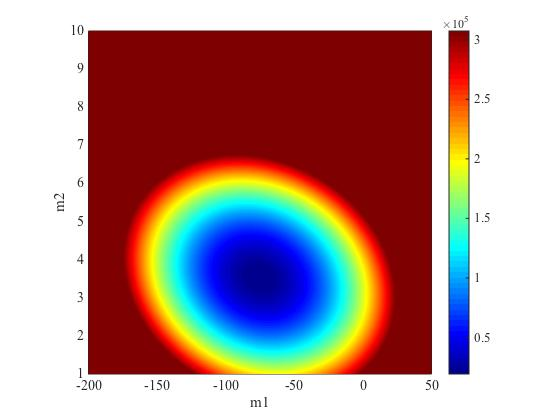
\includegraphics[scale=0.5]{p1_figures/errorellip}


\subsubsection*{(e)- 10 points}

First calculate the misfit $F(\boldsymbol{m})$ for the full parameter
space.

From Bayesian law and uniform prior,

\begin{eqnarray*}
P(\boldsymbol{m}|\boldsymbol{d}) & \propto & P(\boldsymbol{d}|\boldsymbol{m})\\
 & \propto & \exp(-F(\boldsymbol{m}))\\
\end{eqnarray*}


Normalize the pdf so its integral over the model space equals 1.

\begin{eqnarray*}
P(\boldsymbol{m}|\boldsymbol{d}) & = & \frac{\exp(-F(\boldsymbol{m}))}{\int\exp(F(\boldsymbol{m}))d\boldsymbol{m}}
\end{eqnarray*}


that is

\begin{eqnarray*}
P(m_{1},m_{2}|\boldsymbol{d}) & = & \frac{\exp(-F(m_{1},m_{2}))}{\int\int P(m_{1},m_{2}|d)dm_{1}dm_{2}}
\end{eqnarray*}


The marginals are: 
\begin{eqnarray*}
P(m_{1}|d) & = & \int P(m_{1},m_{2}|d)dm_{2}\\
P(m_{2}|d) & = & \int P(m_{1},m_{2}|d)dm_{1}\\
\end{eqnarray*}


We can approximate the integral with rectangle method: $\int f(x)dx=\sum_{i}f(x_{i})\triangle x$.

(1) Result using given data error $\sigma=0.1$

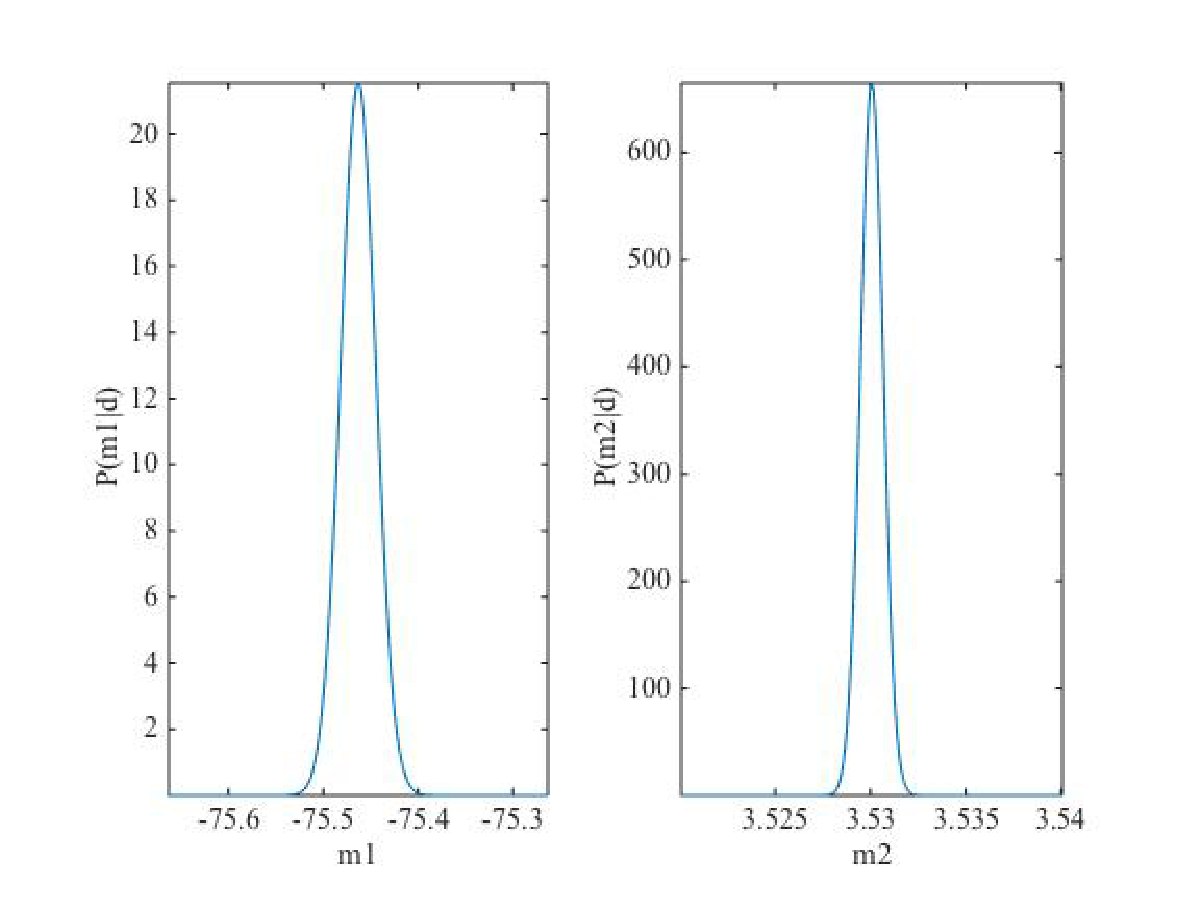
\includegraphics[scale=0.7]{p1_figures/margin}

(2) Result using estimated data error $s=26.3$

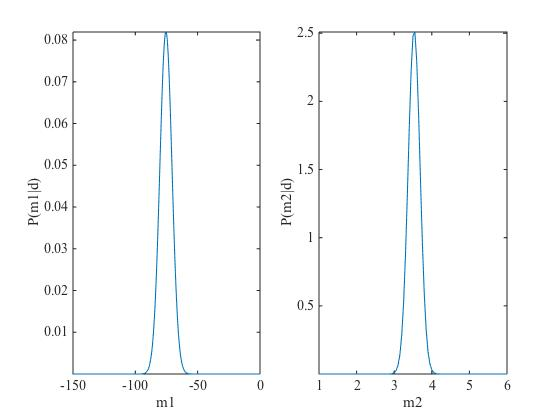
\includegraphics[scale=0.7]{p1_figures/margins}


\subsubsection*{(f)- 8 points}

By definition

\begin{eqnarray*}
\sigma_{m_{i}}^{2}=E[m_{i}^{2}]-(E[m_{i}])^{2} & = & \int p(m_{i}|d)m_{i}^{2}dm_{i}-\left(\int p(m_{i}|d)m_{i}dm_{i}\right)
\end{eqnarray*}


(see MATLAB code) 

(1) Result using given data error $\sigma=0.1$

We get $\sigma_{m1}=0.0185$, $\sigma_{m2}=0.0006$, which are very
close to square root of the diagonal elements of the covariance matrix
calculated in (c).

(2) Result using estimated data error $s=26.3$

We get $\sigma_{m1}=4.8692$, $\sigma_{m2}=0.1577$, which are very
close to square root of the diagonal elements of the covariance matrix
calculated in (c).


\subsubsection*{MATLAB code for (a)-(b)}

\tiny
\lstinputlisting{p1/hw2_1.m}
\normalsize


\subsubsection*{MATLAB code for (c)-(f)}

\tiny
\lstinputlisting{p1_2/hw2_2s.m}
\normalsize

\newpage{}


\subsection*{Problem 2 (graded by Kangchen) - 50 points}


\subsubsection*{(a) - 5 points}

It is not reasonable to assume that all model parameters have constant
priors (-$\infty$ to $\infty$). For $x_{s}$and $y_{s}$, we should
know that it cannot be too far from where the volcano is. For $z_{s}$
which we defined as depth, it must be positive. For P which is related
to pressure, we know that it must be positive too.


\subsubsection*{(b) - 10 points}

We can incorporate this information as a prior by multiplying our
likelihood $P(\{d_{k}\}|\boldsymbol{m})$ by a prior for the model
$P(\boldsymbol{m})$. In this case we will use a Gaussian distribution
for model parameter $p$ with $\mu=35$ and $\sigma=6$.

\begin{eqnarray*}
P(\boldsymbol{m})=e^{-\frac{1}{2}(\frac{p-\mu}{\sigma})^{2}}\\
P(\boldsymbol{m}|\{d_{k}\})=P(\{d_{k}\}|\boldsymbol{m})P(\boldsymbol{m})\\
P(\boldsymbol{m}|\{d_{k}\})=e^{-F(\boldsymbol{m})}e^{-\frac{1}{2}(\frac{p-\mu}{\sigma})^{2}}\\
P(\boldsymbol{m}|\{d_{k}\})=e^{-F(\boldsymbol{m})-\frac{1}{2}(\frac{p-\mu}{\sigma})^{2}}
\end{eqnarray*}



\subsubsection*{(c.i) - 5 points}

\begin{eqnarray*}
\int_{\phi_{1}}^{\phi_{2}}{P(\phi)d\phi}=\int_{\phi_{1}}^{\phi_{2}}{\frac{1}{\phi}d\phi}=\ln(\phi_{2})-\ln(\phi_{1})\\
\int_{k\phi_{1}}^{k\phi_{2}}{P(\phi)d\phi}=\int_{k\phi_{1}}^{k\phi_{2}}{\frac{1}{\phi}d\phi}=\ln(k\phi_{2})-\ln(k\phi_{1})\\
=\ln(k)+\ln(\phi_{2})-\ln(k)-\ln(\phi_{1})\\
=\ln(\phi_{2})-\ln(\phi_{1})
\end{eqnarray*}


So $P(\phi)=\frac{1}{\phi}$ satisfies the scale independent criterion.


\subsubsection*{(c.ii) - 5 points}

We can again incorporate this information as a prior in our expression
for $P(\boldsymbol{m}|\{d_{k}\})$ by multiplying it times our likelihood
(just like in part b). Our expresssion becomes:

\begin{eqnarray*}
P(\boldsymbol{m}|\{d_{k}\})=e^{-F(\boldsymbol{m})}\frac{1}{p}=e^{-F(\boldsymbol{m})-ln(p)}
\end{eqnarray*}



\subsubsection*{(d) - 5 points}

We want to incorporate both independent pieces of information into
our prior. In this case we can multiply the two priors together. Our
new expression becomes:

\begin{eqnarray*}
P(\boldsymbol{m}|\{d_{k}\})=\frac{1}{p}e^{-F(\boldsymbol{m})}e^{-\frac{1}{2}(\frac{p-\mu}{\sigma})^{2}}=e^{-F_{old}(\boldsymbol{m})-\frac{1}{2}(\frac{p-\mu}{\sigma})^{2}-\ln(p)}
\end{eqnarray*}


Let's plot the two priors separately and then together to see which
information dominates the result. Figure 0.1 is the Gaussian prior.
Figure 0.2 is the scale independent prior. Figure 0.3 is their combination.
We can see that the Gaussian prior is scaled by the scale invariant
prior, but still mainly retains it's shape and thus dominates the
result. This is primarily because the scale invariant prior is nearly
constant over the range of $p$ that the Gaussian is significantly
non-zero.

\begin{figure}
\centering{}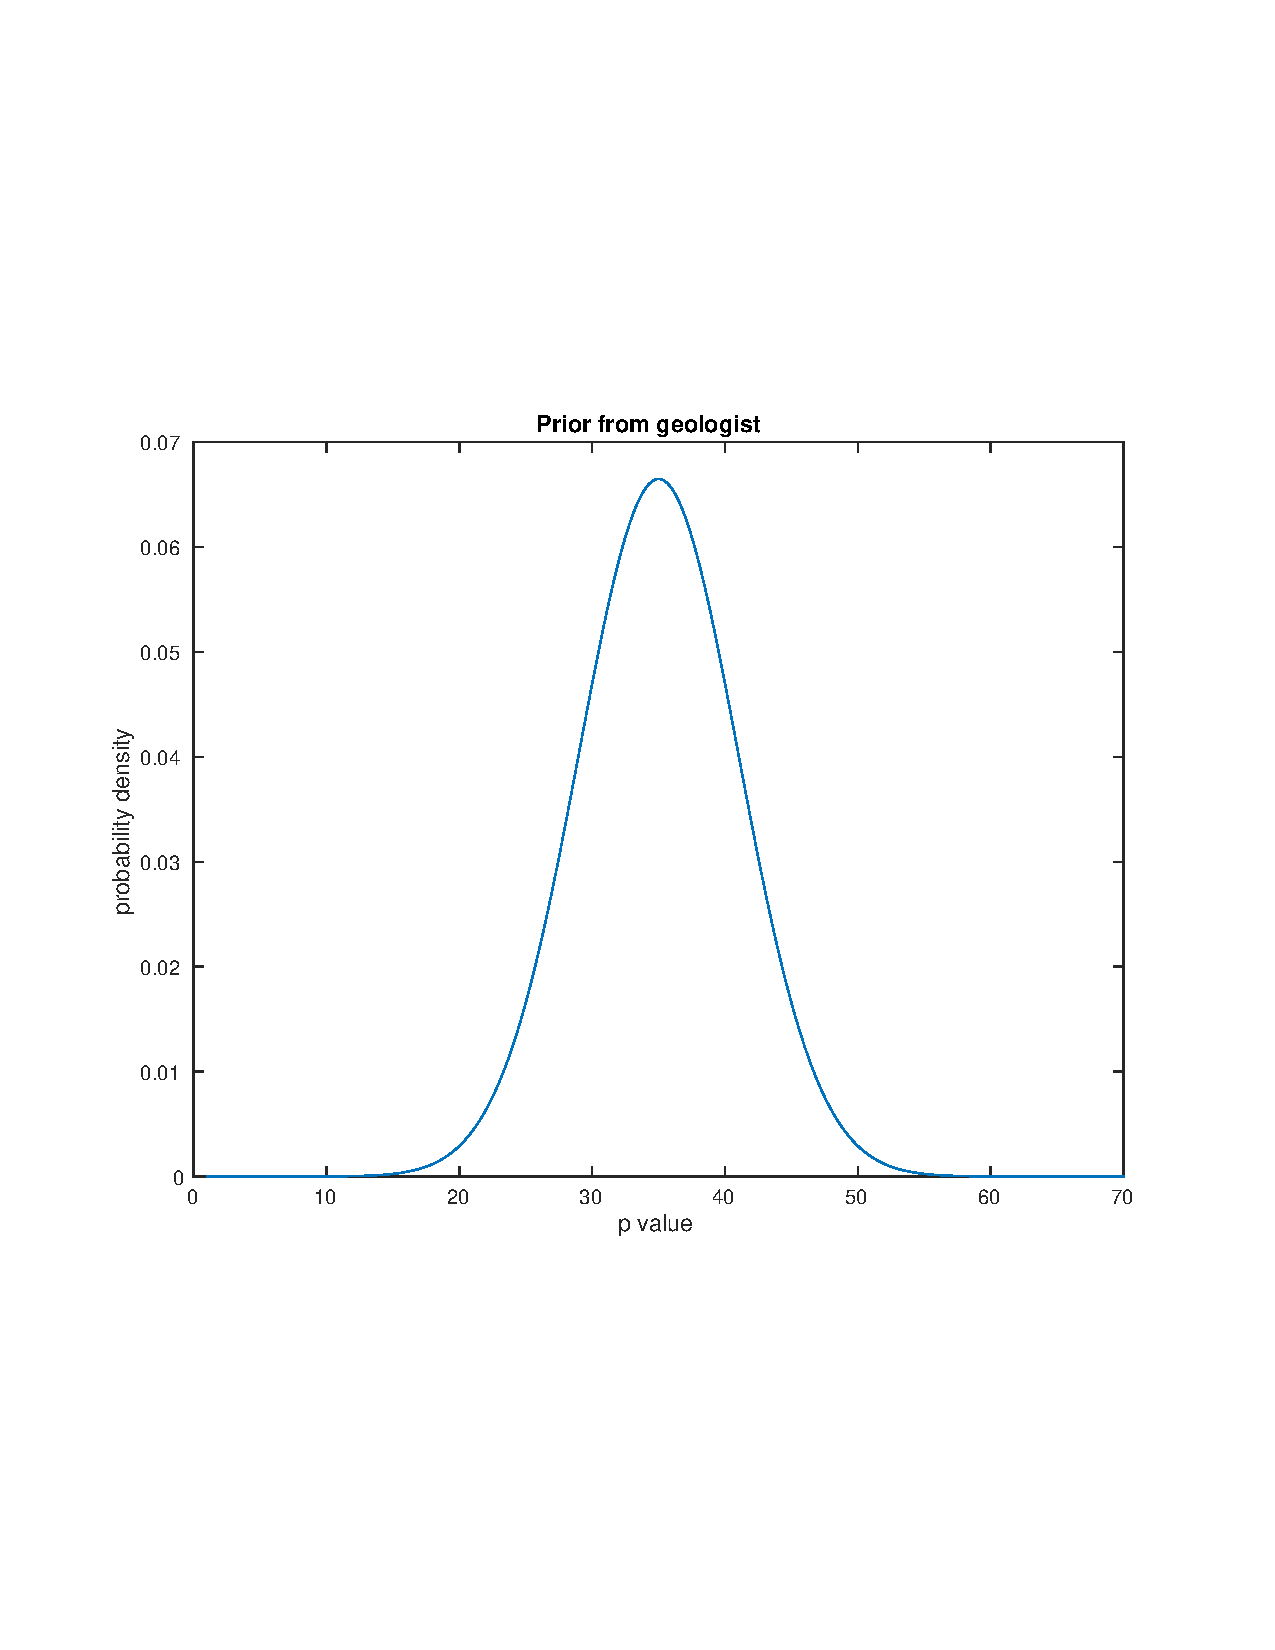
\includegraphics[width=12cm]{Q2/Geo_prior} \caption{Plot of the Gaussian prior for p.}
\end{figure}


\begin{figure}
\centering{}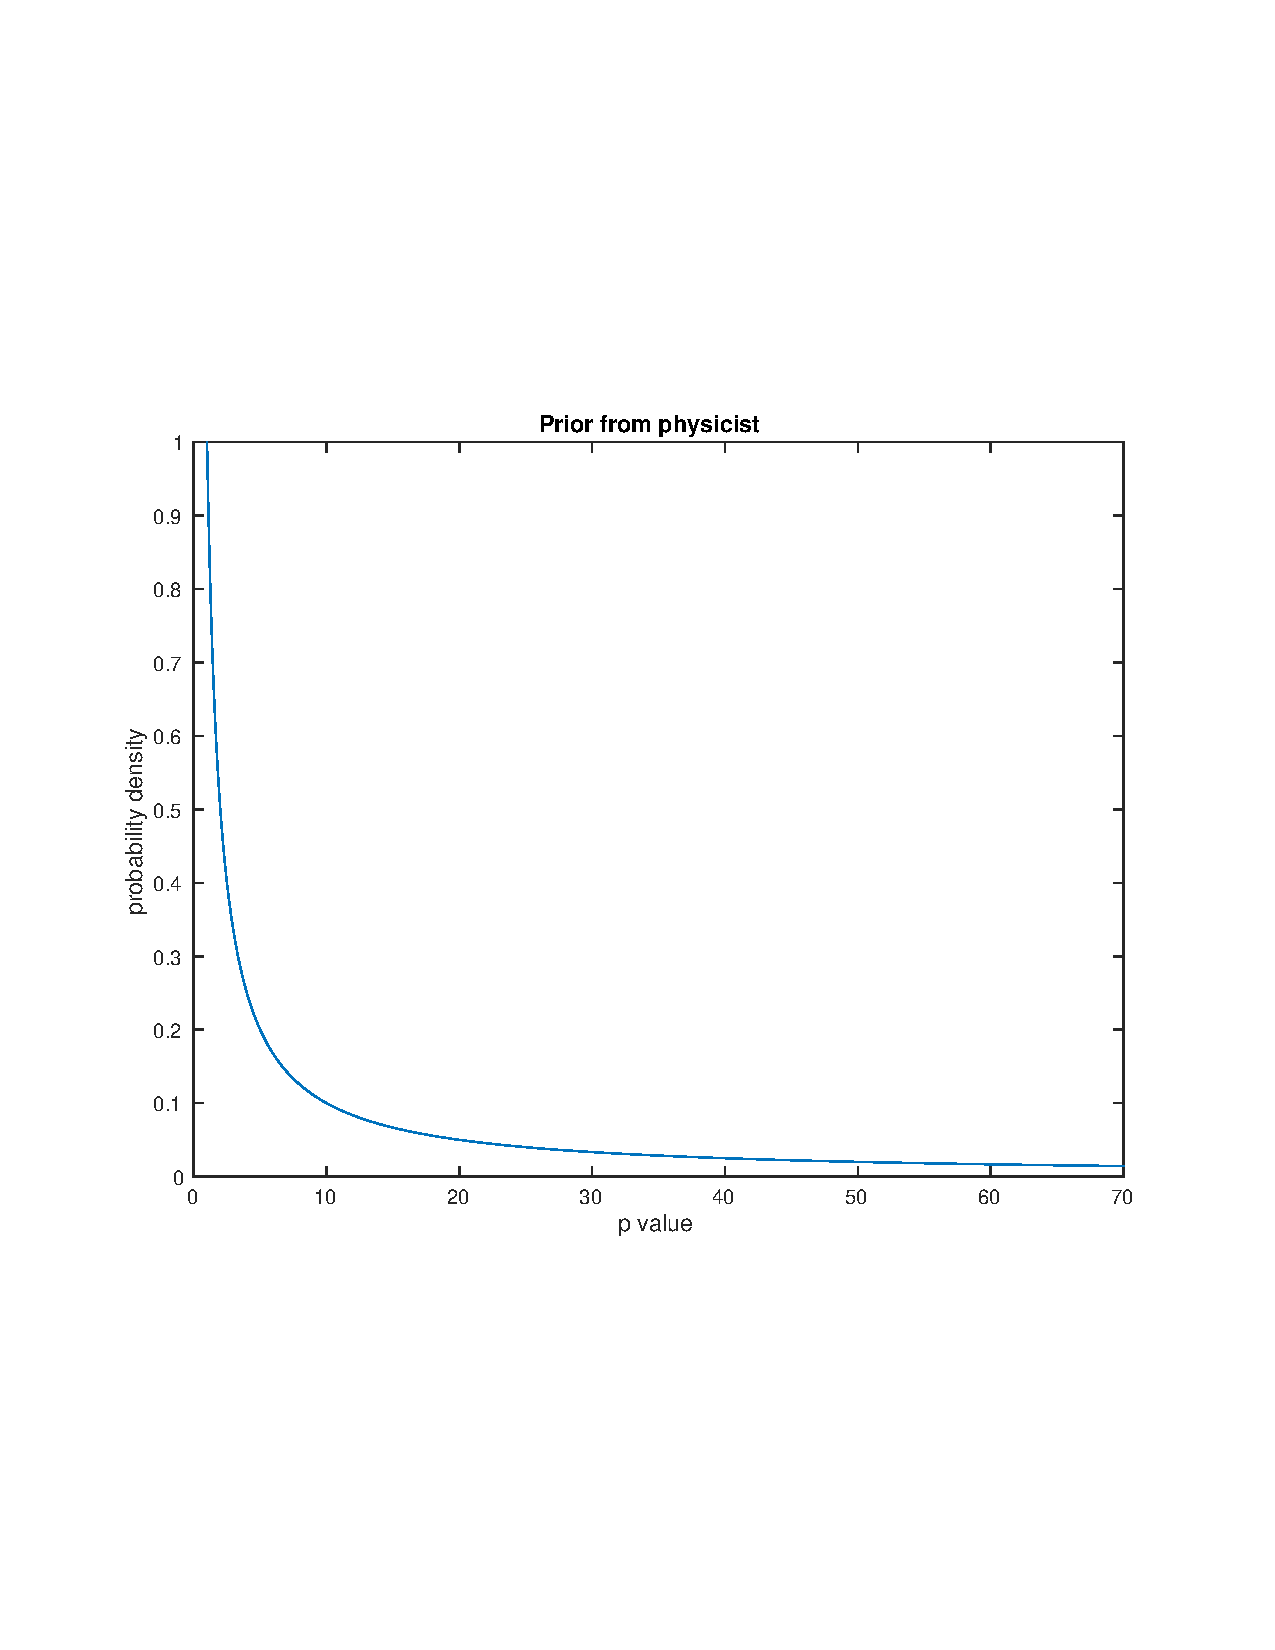
\includegraphics[width=12cm]{Q2/Phy_prior} \caption{Plot of the scale invariant prior for p.}
\end{figure}


\begin{figure}
\centering{}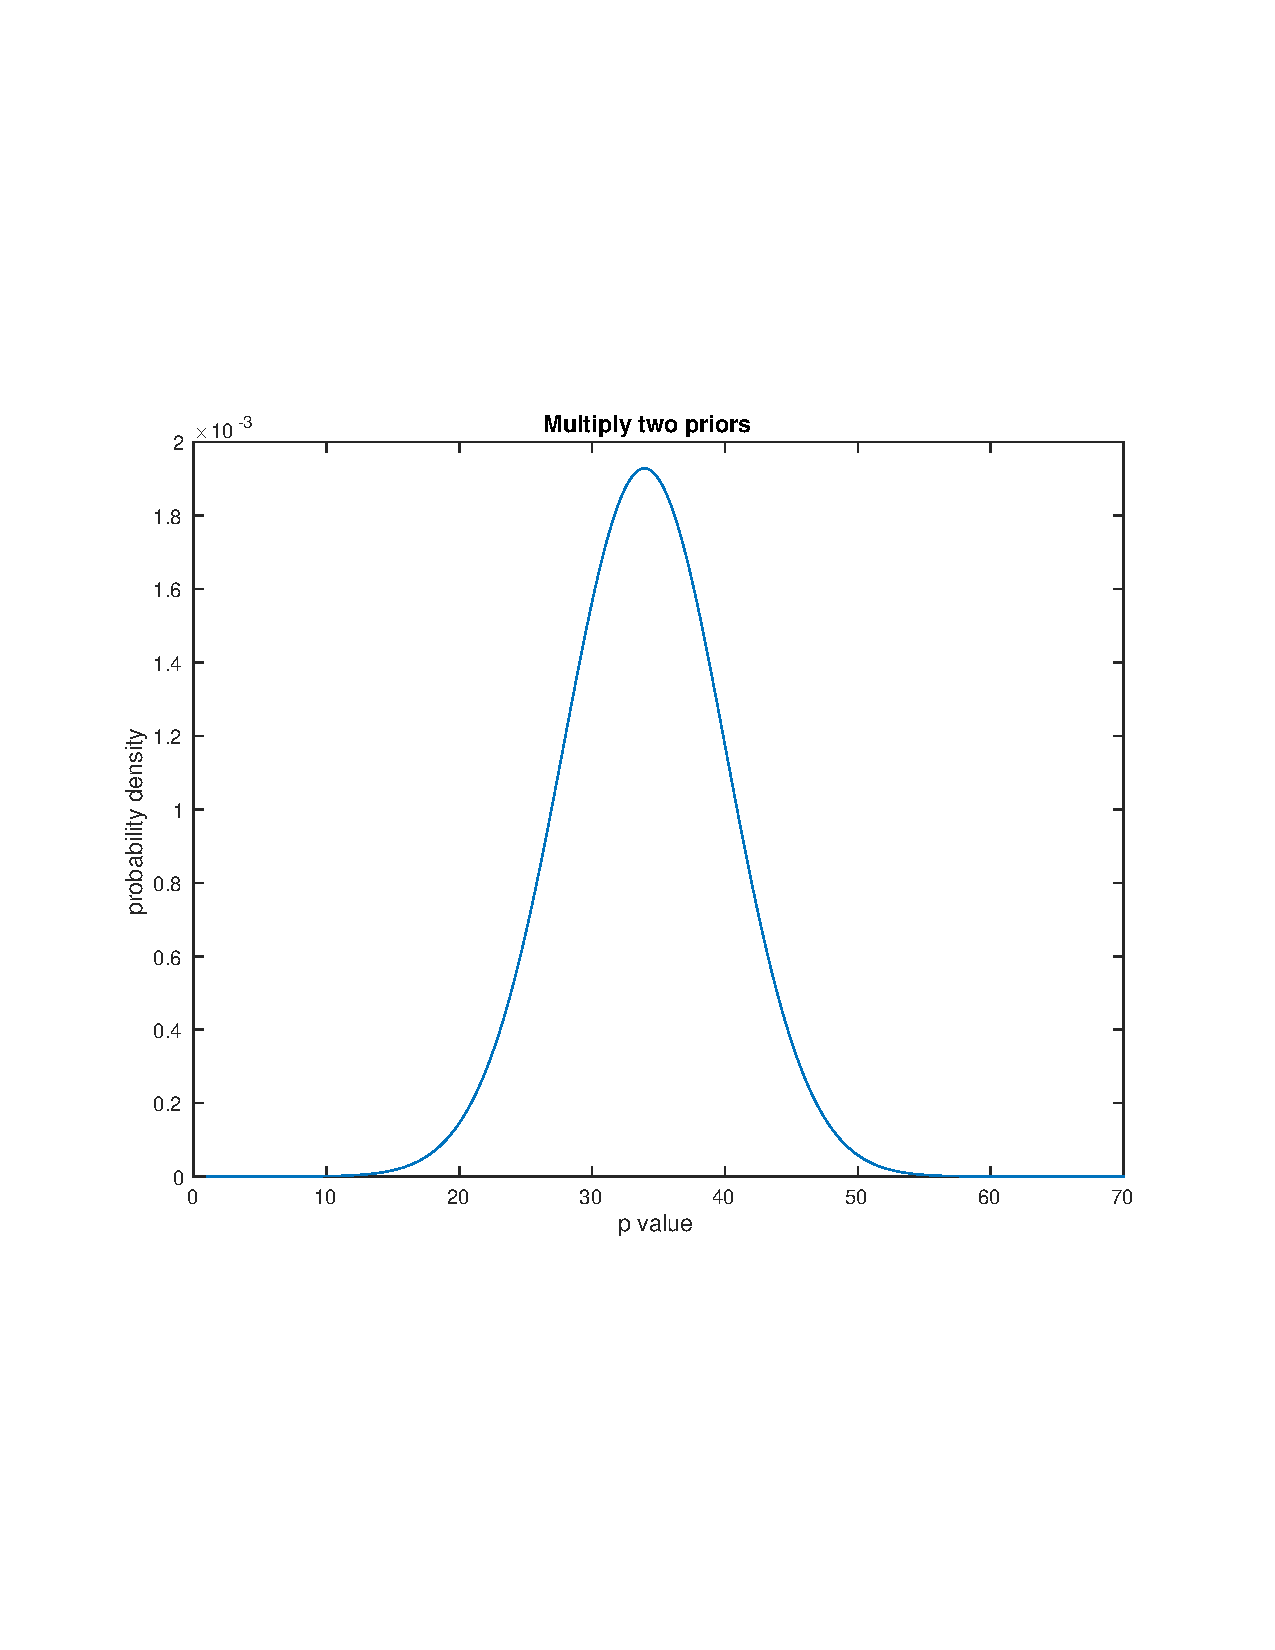
\includegraphics[width=12cm]{Q2/MUl_prior} \caption{Plot of combination of the Gaussian and scale invariant priors for
p. }
\end{figure}



\subsubsection*{(e) - 5 points}

It doesn't matter in what order we do things as long as priors for
analysis are not biased by our data (and they shouldn't be) and your
experiment is not affected by prior information. An example of a situation
in which the experiment is affected by prior is that if we have some
prior information about $x_{s}$ and $y_{s}$ which is not the case
here, we can conduct our mesasurements closer to those prior points
which may increase accuracy of our inversion.


\subsubsection*{(f) - 15 points}

Previous expression: $P_{old}(\boldsymbol{m}|\{d_{k}\})=e^{-F_{old}(\boldsymbol{m})}$
\\
 New expression: $P(\boldsymbol{m}|\{d_{k}\})=\frac{1}{p}e^{-F_{old}(\boldsymbol{m})}e^{-\frac{1}{2}(\frac{p-\mu}{\sigma})^{2}}$
\\


Previous misfit function: $F_{old}(\boldsymbol{m})$ \\
 To find the new misfit function we will need to manipulate our expression
to get everything into a single exponential. Let's start with the
$\frac{1}{p}$ part:

\begin{eqnarray*}
\frac{1}{p}=e^{(\ln(\frac{1}{p})}=e^{-\ln(p)}\\
P(\boldsymbol{m}|\{d_{k}\})=e^{-\ln(p)}e^{-F_{old}(\boldsymbol{m})}e^{-\frac{1}{2}(\frac{p-\mu}{\sigma})^{2}}\\
\end{eqnarray*}


New misfit function: $F(\boldsymbol{m})=F_{old}(\boldsymbol{m})+\ln(p)+\frac{1}{2}(\frac{p-35}{6})^{2}$
\\


We only need to make a couple simple changes to our code from HW2.
Instead of just using the L2 norm as our error function, we now need
to add our extra two terms to our misfit function:

We will add a term to the last entries of $\gamma$ and the Hessian
to account for the new priors on $p$.

Add the first derivative of our new part of the misfit to $\gamma$:

\begin{eqnarray*}
\gamma=\gamma_{old}-\frac{1}{p}-\frac{p-\mu}{\sigma^{2}}
\end{eqnarray*}


And the second derivative to the last entry of the Hessian:

\begin{eqnarray*}
\frac{\partial^{2}F}{\partial p^{2}}=\frac{\partial^{2}F_{old}}{\partial p^{2}}+\frac{-1}{p^{2}}+\frac{1}{\sigma^{2}}
\end{eqnarray*}


Here is the full code: 


\subsection*{\tiny
\lstinputlisting{./Q2/HW2.m}
\normalsize\tiny
\lstinputlisting{./Q2/compute_gradient_approx_hess.m}
\normalsize\tiny
\lstinputlisting{./Q2/nonlinear_solver.m}
\normalsize\tiny
\lstinputlisting{./Q2/compute_misfit.m}
\normalsize}

Our best fit solution is now:
\[
\begin{bmatrix}x_{s}\\
y_{s}\\
z_{s}\\
p
\end{bmatrix}=\begin{bmatrix}8.5332\\
-5.7685\\
12.1910\\
33.9391
\end{bmatrix}
\]


Comparing with old solution, the new solution has $p$ value closer
to $35$ which is given by geologist's prior.\newpage{}


\subsection*{Problem 3 (graded by Kangchen) - bonus 15 points}


\subsubsection*{(a)-5 points}

The posterior probability is given by 
\begin{equation}
p(\mu|x)\propto\left(\sum_{k=1}^{N}(x_{k}-\mu)^{2}\right)^{-\frac{N-1}{2}}=\exp\left(-\frac{N-1}{2}\ln\left[\sum_{k=1}^{N}(x_{k}-\mu)^{2}\right]\right).
\end{equation}
Minima of $F$ maximize the probability density function. We have
that 
\begin{align}
F(\mu) & =\frac{N-1}{2}\ln\left(\sum_{k=1}^{N}(x_{k}-\mu)^{2}\right),\\
\frac{\partial F}{\partial\mu} & =-(N-1)\frac{\sum_{k=1}^{N}(x_{k}-\mu)}{\sum_{k=1}^{N}(x_{k}-\mu)^{2}}\\
\frac{\partial^{2}F}{\partial\mu^{2}} & =(N-1)\frac{N\sum_{k=1}^{N}(x_{k}-\mu)^{2}-2(\sum_{k=1}^{N}(x_{k}-\mu))^{2}}{\left(\sum_{k=1}^{N}(x_{k}-\mu)^{2}\right)^{2}}.
\end{align}
Taking the derivative with respect to $\mu$ and setting it to zero
yields the minimum $\mu_{0}$

\[
\frac{\partial F}{\partial\mu}=-(N-1)\frac{\sum_{k=1}^{N}(x_{k}-\mu)}{\sum_{k=1}^{N}(x_{k}-\mu)^{2}}=0
\]
 

Because $\sum_{k=1}^{N}(x_{k}-\mu)^{2}>0$, we have $\sum_{k=1}^{N}(x_{k}-\mu)=0$

\begin{equation}
\mu_{0}=\frac{1}{N}\sum_{k=1}^{N}x_{k},
\end{equation}
For the second derivative at the best fit solution we have

\begin{align}
\frac{\partial^{2}F}{\partial\mu^{2}}(\mu=\mu_{0}) & =(N-1)\frac{N\sum_{k=1}^{N}(x_{k}-\mu_{0})^{2}-2(\sum_{k=1}^{N}(x_{k}-\mu_{0}))^{2}}{\left(\sum_{k=1}^{N}(x_{k}-\mu_{0})^{2}\right)^{2}}\\
 & =(N-1)\frac{N\sum_{k=1}^{N}(x_{k}-\mu_{0})^{2}-2(\sum_{k=1}^{N}(x_{k}-\frac{1}{N}\sum_{k=1}^{N}x_{k}))^{2}}{\left(\sum_{k=1}^{N}(x_{k}-\mu_{0})^{2}\right)^{2}}\\
 & =(N-1)\frac{N\sum_{k=1}^{N}(x_{k}-\mu_{0})^{2}}{\left(\sum_{k=1}^{N}(x_{k}-\mu_{0})^{2}\right)^{2}}\\
 & =\frac{N(N-1)}{\sum_{k=1}^{N}(x_{k}-\mu_{0})^{2}}
\end{align}


The standard deviation $\sigma_{\mu}$ then amounts to 
\begin{equation}
\sigma_{\mu}=\frac{1}{F''(\mu_{0})^{1/2}}=\frac{S}{\sqrt{N}},
\end{equation}
where 
\begin{equation}
S=\sqrt{\frac{1}{N-1}\sum_{k=1}^{N}(x_{k}-\mu_{0})^{2}}
\end{equation}
is the sample variance of the data.


\subsubsection*{(b)-5 points}

We assume $\boldsymbol{Q}=[\boldsymbol{e}_{1},\boldsymbol{e}_{2}]$
where $||\boldsymbol{e}_{1}||=1,$$||\boldsymbol{e}_{2}||=1$. We
can write $\boldsymbol{e}_{1}=(cos(\theta),sin(\theta))^{T}$ and
$\boldsymbol{e}_{2}=(cos(\phi),sin(\phi))^{T}.$ Since $\boldsymbol{Q}$
is an orthongonal matrix, $\boldsymbol{e}_{1}$ and $\boldsymbol{e}_{2}$
are orthogonal. That means $cos(\theta)cos(\phi)+sin(\theta)sin(\phi)=cos(\theta-\phi)=0$.
So $\theta-\phi=\pi/2$ or $-\pi/2$. If we assume that $\phi=\theta+\pi/2$,
then $\boldsymbol{Q}=\begin{bmatrix}cos(\theta) & -sin(\theta)\\
sin(\theta) & cos(\theta)
\end{bmatrix}$. This can be understood as rotating a vector by $\theta$ degree
counterclockwise. Another way to interpret what $\boldsymbol{Q}$
did is that $\boldsymbol{Q}^{T}\begin{pmatrix}x\\
y
\end{pmatrix}$ gives the projection of $\begin{pmatrix}x\\
y
\end{pmatrix}$ onto $\boldsymbol{e}_{1}$ and $\boldsymbol{e}_{2}$ where $\boldsymbol{Q}=(\boldsymbol{e}_{1},\boldsymbol{e}_{2}).$


\subsubsection*{(c)-5 points}

We need to show that $\sigma_{x}^{2}=\frac{B}{AB-C^{2}}$. We are
dealing with an integral of the f
\begin{align}
\sigma_{x}^{2} & =\frac{\int_{-\infty}^{+\infty}\int_{-\infty}^{+\infty}dxdy\,x^{2}\exp\left(-\frac{1}{2}x^{T}Ax\right)}{\int_{-\infty}^{+\infty}\int_{-\infty}^{+\infty}dxdy\,\exp\left(-\frac{1}{2}x^{T}Ax\right)}\\
 & =\frac{\int_{-\infty}^{+\infty}\int_{-\infty}^{+\infty}dxdy\,x^{2}\exp\left(-\frac{1}{2}(Ax^{2}+2Cxy+By^{2})\right)}{\int_{-\infty}^{+\infty}\int_{-\infty}^{+\infty}dxdy\,\exp\left(-\frac{1}{2}(Ax^{2}+2Cxy+By^{2})\right)}\\
 & =\frac{\int_{-\infty}^{+\infty}\int_{-\infty}^{+\infty}dxdy\,x^{2}\exp\left(-\frac{1}{2}(A-C^{2}/B)x^{2}-\frac{1}{2}B(y+Cx/B)^{2}\right)}{\int_{-\infty}^{+\infty}\int_{-\infty}^{+\infty}dxdy\,\exp\left(-\frac{1}{2}(A-C^{2}/B)x^{2}-\frac{1}{2}B(y+Cx/B)^{2}\right)}\\
 & =\frac{\int_{-\infty}^{+\infty}dx\,x^{2}\exp\left(-\frac{1}{2}(A-C^{2}/B)x^{2}\right)\mbox{\ensuremath{\int_{-\infty}^{+\infty}}\ensuremath{dy}exp}\left(-\frac{1}{2}B(y+Cx/B)^{2}\right)}{\int_{-\infty}^{+\infty}dx\,\exp\left(-\frac{1}{2}(A-C^{2}/B)x^{2}\right)\mbox{\ensuremath{\int_{-\infty}^{+\infty}}\ensuremath{dy}exp}\left(-\frac{1}{2}B(y+Cx/B)^{2}\right)}\\
 & =\frac{\int_{-\infty}^{+\infty}dx\,x^{2}\exp\left(-\frac{1}{2}(A-C^{2}/B)x^{2}\right)}{\int_{-\infty}^{+\infty}dx\,\exp\left(-\frac{1}{2}(A-C^{2}/B)x^{2}\right)}
\end{align}


Note that from 0.15 to 0.16:

$\int_{-\infty}^{+\infty}dy\exp\left(-\frac{1}{2}B(y+Cx/B)^{2}\right)=\int_{-\infty+cx/B}^{+\infty+cx/B}dy'\exp\left(-\frac{1}{2}By'{}^{2}\right)=\int_{-\infty}^{+\infty}dy'\exp\left(-\frac{1}{2}By'^{2}\right)$ 

So that integral is not related to $x.$ That's why we can cancel
out that term from both numerator and denominator.

If we set $\sigma^{2}=1/(A-C^{2}/B)$, we arrive at 
\begin{equation}
\sigma_{x}^{2}=\frac{\int dx\,x^{2}\exp\left(-\frac{1}{2}x^{2}/\sigma^{2}\right)}{\int dx\,\exp\left(-\frac{1}{2}x^{2}/\sigma^{2}\right)}
\end{equation}
, which as we have seen in previous homework sets and solutions implies
\begin{equation}
\sigma_{x}^{2}=\langle x^{2}\rangle=\sigma^{2}=\frac{1}{A-\frac{C^{2}}{B}}=\frac{B}{AB-C^{2}}.
\end{equation}
\clearpage{}
\end{document}
